\documentclass[a4paper]{article}

\usepackage[english, serbian]{babel}
\usepackage[utf8]{inputenc}
\usepackage{csquotes}
\usepackage{authblk}
\usepackage{graphicx}
\usepackage{xcolor}
\usepackage{amsmath}
\usepackage{amssymb}
\usepackage{amsfonts}
\usepackage{tabularx}
\usepackage{enumitem}
\usepackage{multicol}
\usepackage{hyperref}

\usepackage[backend=bibtex, style=numeric]{biblatex}
\addbibresource{references.bib}

\graphicspath{ {images/} }

\title{Automatsko prevođenje}
\author{Vladimir Vuksanović}
\affil{Matematički fakultet, Beograd}
\date{}

\begin{document}

\maketitle

\tableofcontents

\newpage

% Uvodni deo koji sadrži opis problema koji se rešava sa pregledom literature i naučne doprinose drugih istraživača na polju rešavanja razmatranog problema.
\section{Uvod}

Automatsko prevođenje podrazumeva prevođenje teksta sa jednog prirodnog jezika na drugi korišćenjem kompjutera.
Preciznije, potrebno je za ulaznu rečenicu proizvoljne dužine na izvornom jeziku generisati izlaznu rečenicu, ne nužno iste dužine, na ciljnom jeziku koja ima isto značenje kao ulazna.

Klasičan način rešavanja ovog problema je statistički zasnovan, SMT (Statistical Machine Translation), pristup koji je bio dominantan decenijama i davao je prilično dobre rezultate. Međutim, u poslednjih nekoliko godina fokus je prešao na modele zasnovane na neuronskim mrežama, prvo kao dopuna SMT modelima pa onda i kao odvojenu paradigmu koja je eventualno uspela da nadmaši klasične pristupe.

U ovom radu će biti predstavljena pojednostavljena varijanta modela za prevođenje zasnovanog na neuronskim mrežama opisanog u \cite{sutskever2014sequence} koji jedan od prvih radova u kome je predložena enkoder-dekoder arhitektura koja se i danas najčešće primenjuje.

% Opis vašeg rešenja zadatog problema. Ovim poglavljem opišite sve relevantne aspekte vašeg rada: npr. opšti rad algoritma, način kodiranja rešenja i funkciju cilja u slučaju da radite optimizacionu tehniku, itd. Budite objektivni i pošteni u opisu svoje metode i jasno ukažite na to da ste reprodukovali pristup koji je neko već osmislio pre vas tako što ćete ubaciti odgovarajuće reference ka svim relevantnim radovima (ovo je potpuno normalna situacija i ne podrazumeva nikakvo smanjivanje poena).
\section {Rešenje}

Za rešavanje ovog problema ćemo koristiti NMT (Neural Machine Translation) pristup koji koristi neuronsku mrežu da predvidi sekvencu reči u prevodu. 
Kako su ulaz i izlaz sekvence koje mogu biti proizvoljnih dužina, prevođenje pripada grupi sequence-to-sequence problema. To onemogućava korišćenje potpuno povezane mreže jer ona zahteva fiksan broj ulaza i izlaza. 
Umesto toga, moderan pristup koristi enkoder-dekoder arhitekturu opisanu u \cite{sutskever2014sequence} i \cite{cho2014learning} u kombinaciji sa rekurentnim neuronskim mrežama (LSTM ili GRU).
Ova arhitektura u praksi daje veoma dobre rezultate zbog čega je i koristi jedan od najpoznatijih servisa ovog tipa, \href{https://translate.google.com/}{Google Translate} \cite{wu2016googles}. 

Osnovna ideja je da se model podeli na dva dela.
Prvi deo, enkoder, prima ulaz reč po reč (ili slovo po slovo), svaku od njih prosleđuje LSTM sloju i na osnovu toga generiše reprezentaciju \textit{fiksne} dužine koja sadrži iste informacije kao polazna rečenica samo mapirana u novi prostor.
Ta reprezentacija se zatim prosleđuje drugom delu, dekoderu, kao polazna tačka za generisanje prevoda na ciljni jezik analognim postupkom, reč po reč. U svakom koraku ulaz u dekoder čine trenutno stanje LSTM sloja i poslednja generisana reč.
Na početku ta reč je poseban token za početak rečenice, a reči se generisu sve dok se ne dođe do tokena za kraj prevoda ili do zadate maksimalne dužine.

Originalni rad je predložio da se obrtanjem redosleda reči u ulaznim rečenicama bolje očuvaju veze između reči, ali kako su rečenice na kojima je ovaj model treniran kratke, ovaj doprinos se ne primećuje i neće biti korišćen.

\section{Implementacija}

Model je implementiran u programskom jeziku Python uz korišćenje \href{https://keras.io/}{keras} biblioteke. Implementacija prati osnovne korake sa zvaničnog sequence-to-sequence primera sa keras veb stranice \cite{keras_seq2seq} pri čemu se predikcija vrši na nivou reči umesto pojedinačnih slova.
U nastavku će biti opisan postupak pretprocesiranja i građenja modela za treniranje i predviđanje zajedno sa parametrima koji su korišćeni za treniranje.

\subsection{Pretprocesiranje}

Podaci za trening se sastoje od rečenica na izvornom jeziku i njihovih prevoda na ciljni jezik.
Pre njihove obrade, izbačeni su svi parovi koji imaju isti ulaz a drugačiji prevod. Ovo je odrađeno zato što skup podataka sadrži veliki broj duplikata koji međusobno ometaju jedni druge.

Pošto direktna upotreba rečenica u tekstualnom obliku nije pogodna, potrebno je pretvoriti ih u reprezentaciju koja bolje radi sa neuronskom mrežama.
Prvi korak pretprocesiranja je eliminisanje specijalnih simbola iz rečenica jer nam oni nisu korisni prilikom prevođenja.
Zatim, kako bi rečenice mogle da se upotrebe kao ulaz neuronske mreze potrebno je predstaviti ih kao niz brojeva. To se radi jednostavnim pridruživanjem broja svakoj reči iz trening skupa ili nekog predefinisanog rečnika u kom slučaju se dodaje i token za nepoznate (out-of-vocabulary) reči. Ovaj proces se naziva tokenzacija i radi se odvojeno za ulaz i izlaz.
Za velike trening skupove bi bilo bolje ograničiti skup reči na rečnik, ali ovde je korišćen pristup sa svim rečima iz trening skupa.

Originalni papir predlaže dodatno da se za ulazne rečenice obrne redosled tokena u sekvenci zato što se tako bolje očuvaju veze između reči u dužim rečenicama. Zbog kratkih rečenica u trening skupu, ovu tehniku nećemo primeniti, ali je ostavljena kao opcija u kodu.

Dalje, potrebno je napraviti dva tipa izlaznih rečenica, jedan tip predstavlja ulaz u dekoder a drugi predstavlja izlaz. Prva reč koju dekoder treba da dobije je početni (start of sequence) token i on se dodaje na početak svake rečenice koja ulazi u dekoder. Slično, na rečenice koje predstavljaju izlaz iz dekodera potrebno je dodati završni (end of sequence) token.

Sve sekvence iz respektivnih skupova se potom dopunjavaju "praznim" tokenima tako da budu iste dužine. Pri tome, ulazne sekvence se dopunjuju sa leve strane jer se konačan rezultat dobija pri izlazu poslednjeg tokena, a izlazne sekvence se dopunjuju sa desne strane jer njihova obrada počinje prvim tokenom.
Ovim smo dobili skup ulazno-izlaznih sekvenci koje mogu da se koriste za treniranje neuronske mreže.

\subsection{Enkoder}

Enkoder je zadužen da na osnovu dobijene sekvence generiše reprezentaciju fiksne dužine koja bi trebalo da sadrži sve informacije potrebne da se konstruiše prevod na ciljnom jeziku.

Ulaz u enkoder je tensor dimenzije $n \times m$ gde je $n$ broj rečenica, a $m$ dužina ulazne sekvence. On je vezan za embedding sloj koji svakoj reci dodeljuje vektor fiksne dužine tako da udaljenost između vektora zavisi od značenja reči.
Umesto da model uči te reprezentacije za vreme treninga, koristimo \href{https://nlp.stanford.edu/projects/glove/}{GloVe} model \cite{pennington2014glove} treniran na 5 milijardi reči sa vikipedije gde je svaka reč prestavljena vektorom dužine 100. 
Embedding sloj je zatim vezan na LSTM sloj dimenzije 512 koji se inicijalizuje nasumičnim vrednostima iz uniformne raspodele na intervalu $[-0.08, 0.08]$. Kao izlaz iz ovog sloja se dobija njegovo interno stanje na kraju koje prestavlja novu reprezentaciju ulazne rečenice.

\subsection{Dekoder}

Dekoder koristi svoje unutrašnje stanje i prethodno generisanu reč kako bi odredio sledeću reč u rečenici.

Po strukturi, dekoder je veoma sličan enkoderu.
Ulazni sloj sada ima drugu dimenziju jednaku dužini izlazne sekvence dok embedding i LSTM slojevi ostaju nepromenjeni osim sto težine za embedding sloj neće biti unapred zadate nego će se učiti u toku treniranja.
Na kraju se nadovezuje na potpuno povezani sloj sa softmax aktivacijom koji određuje verovatnoću za svaku reč na ciljnom jeziku.

Inicijalno se kao unutrašnje stanje koristi izlaz iz enkodera, a kao prethodno generisanu rec uzimamo početni (\textless sos\textgreater) token koji je uveden prilikom pretprocesiranja. Dekodiranje se prekida ili kada se dobije završni (\textless eos\textgreater) token ili dok se ne dostigne zadata maksimalna dužina rečenice.

\subsection{Model}

Kombinovanjem prethodno opisanih enkodera i dekodera tako da dekoder inicijalno dobije stanja iz enkodera, dobija se konačni model prikazan na slici \ref{fig:model}.

\begin{figure}[h!]
  \centering
    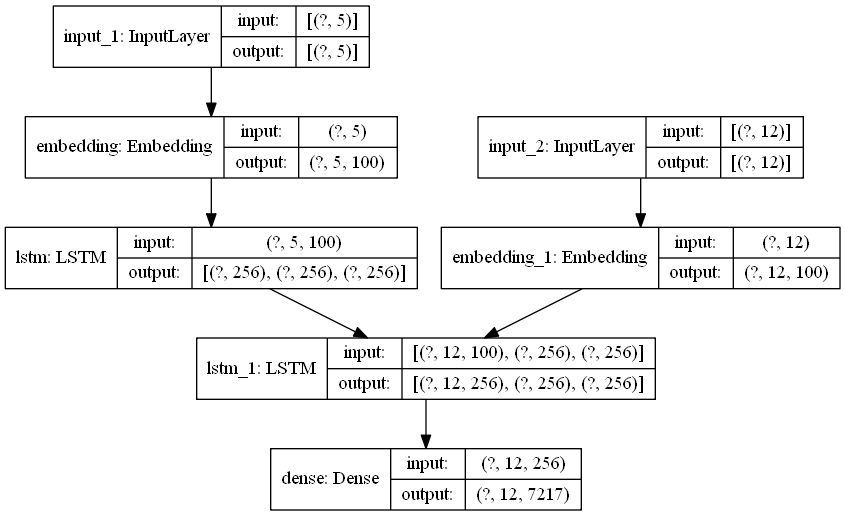
\includegraphics[width=\textwidth]{model}
  \caption{Model za treniranje}
  \label{fig:model}
\end{figure}

Optimizator koji koristimo je \textit{rmsprop}, funkcija gubitka je kategorijska unakrsna entropija, a metrika koju pratimo je tačnost.

\subsection{Trening}

Opisani model je treniran na 50.000 parova rečenica na engleskom i francuskom jeziku iz skupa preuzetog sa \cite{manythings}. Trening je trajao 5 epoha sa veličinom grupe od 128 instanci i 10\% skupa je korišćeno za validaciju. Pošto ceo skup obrađenih podataka ne moze da stane u radnu memoriju za veće brojeve rečenica, korišćen je generator da se grupe rečenica konstruišu tek kada su potrebne.

Za treniranje je korišćena \href{https://colab.research.google.com/}{Google Colaboratory} platforma i trajalo je 2 sata.

\subsection{Generisanje prevoda}

Prethodni model radi samo ako već na samom početku imamo celu prevedenu rečenicu što je dobro za vreme treniranja modela ali je neupotrebljivo za potrebe prevođenja proizvoljnih novih rečenica. Iz tog razloga pravimo novi model koji koristi već trenirane delove iz prethodnog modela ali sa modifikovanim dekoderom.
Ulaz u novi dekoder je samo jedna reč koja se inicijalno postavlja da bude početni token. Sada je moguće iterativno pozivati dekoder sve dok ne dođe do zavrsnog tokena ili nekog unapred određenog limita na dužinu rečenice.
Novi model je prikazan na slici \ref{fig:inference_model}.

\begin{figure}[h!]
  \centering
    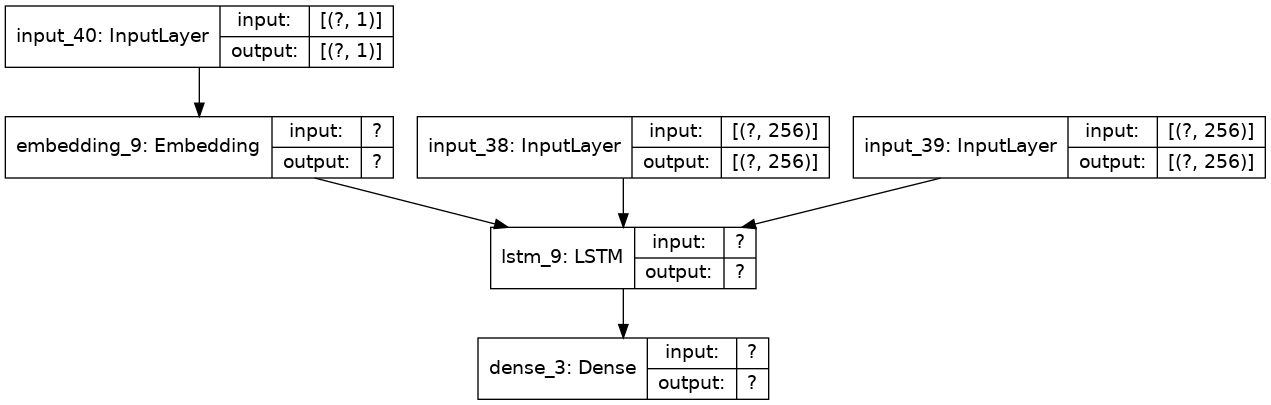
\includegraphics[width=\textwidth]{inference_model}
  \caption{Model za predviđanje}
  \label{fig:inference_model}
\end{figure}

\subsection{Beam search algoritam}

Umesto da se prevod traži gramzivo, uvek gledajući jedan mogući prevod, možemo da dobijemo veliko poboljšanje koristeći \textit{beam search} algoritam koji će heuristički da proveri veći broj prevoda i izabere najbolji među njima.

Prvo se zadaje parametar $k$ koji predstavlja broj rečenica koje će se razmatrati u svakom trenutku. Na početku se bira $k$ reči koje mreža predviđa kao najverovatnije na osnovu vrednosti potpuno povezanog sloja. Kada se izabere prvih $k$ kandidata, svaki od njih se potom dopunjuje svim mogućim rečima i bira se $k$ najverovatnijih sevenci među njima.
Ovaj postupak se ponavlja do kraja svake od sekvenci i onda se za konačan prevod uzima najbolja od njih. Specijalno, za vrednost $k = 1$ postupak se svodi na gramzivu pretragu.

Formalno, algoritam maksimizira vrednost funkcije
$$\arg\max_{y} \prod_{t=1}^{T_y} P(y^{<t>}|X, y^{<1>}, y^{<2>}, ..., y^{<t-1>})$$
Kako su sve verovatnoće između 0 i 1, prethodni proizvod brzo postaje veoma mali broj. Zbog toga se umesto običnog proizvoda koristi suma logaritama.
$$\arg\max_{y} \sum_{t=1}^{T_y} \log P(y^{<t>}|X, y^{<1>}, y^{<2>}, ..., y^{<t-1>})$$
Sada kako je suma logaritama strogo rastuća funkcija, prethodna formula favorizuje što duže rečenice. Da bi kompenzovali za ovo, normalizovaćemo formulu tako što je podelimo sa brojem reči u prevodu. Ovo je konačna formula koju koristimo.
$$\arg\max_{y} \frac{1}{T_y} \sum_{t=1}^{Ty} \log P(y^{<t>}|X, y^{<1>}, y^{<2>}, ..., y^{<t-1>})$$

Od izbora parametra $k$ zavisi koliko potencijalnih prevoda će biti razmatrano i time celokupni kvalitet prevoda. Što je parametar veći, više izbora se razmatra ali se vreme za dobijanje prevoda ekponencijalno povećava. U implementaciji je korišćena vrednost $k = 3$. Više detalja se može naći u \cite{Freitag_2017} i \cite{aritificial2009}.

% Poglavlje sa eksperimentalnim rezultatima sadrži tabele i grafike kojim upoređujete vaš pristup sa drugim pristupima iz literature. Pronaći relevantne test primere (instance) I testirati predloženu metodu (metode) na njima, ukoliko su dostupne. Ako ne možete da dođete do test primera iz literature, kreirajte na osnovu opisa iz radova test primere koji su im slični. Testirajte vaše metode pod sličnim uslovima kao i autori iz literature. Pri demonstraciji rada metode uvek pokazati kako vaša metoda radi na na jednostavnim test primerima koji se mogu vizualizovati. Specijalno, ako ne upoređujete rešenje sa drugim rešenjima, možete komentarisati efikasnost algoritma i procenijvati kvalitet tako što ga upoređujete sa drugim pristupima koje ste sami razvili (npr. algoritmom potpune pretrage, eng. brute-force u slučaju da radite optimizacionu tehniku). Budite objektivni i pošteni u prikazu svojih rezultata i jasno naznačite ako vaš pristup nije bolji (što je vrlo verovatno) od onih koji su predloženi u literaturi. U okviru ovog poglavlja opišite i eksperimentalno okruženje u kojem ste testirali vaš program, karakteristike hardvera, operativni sistem, kompajler, itd.
\section{Rezultati}

\subsection{Primeri prevoda}

\newcommand\translation[4] 
{\begin{center}
  \begin{tabularx}{\textwidth}{ |l|X| } 
    \hline
    Recenica & #1 \\
    \hline
    Tacan prevod & #2 \\
    \hline
    Model (greedy) & #3 \\
    \hline
    Model (beam) & #4 \\
    \hline
  \end{tabularx}
\end{center}}

U nastavku su prikazani primeri prevoda rečenica iz trening skupa gramzivim i beam search algoritmom kao i njihov tačan prevod.

\translation
{What's that dog doing?}
{Que fait ce chien ?}
{de quoi chien est il}
{qu'est ce que ce chien}
\translation
{That boy is smart.}
{Ce garçon est intelligent.}
{ce garçon est intelligent}
{ce garçon est intelligent}
\translation
{Tom tasted the cake.}
{Tom a goûté le gâteau.}
{tom a mangé le gâteau}
{tom a mangé le gâteau}
\translation
{It's like riding a bike.}
{C'est comme le vélo, ça ne s'oublie pas.}
{c'est comme comme comme un vélo}
{c'est comme comme un vélo}
\translation
{You can't bury the truth.}
{Vous ne pouvez pas enterrer la vérité.}
{vous ne pouvez pas les autres}
{vous ne pouvez pas la vérité}
\translation
{I know that I'm rambling.}
{Je sais que je suis incohérent.}
{je sais que c'est un peu}
{je sais que je suis en colère}
\translation
{I neither drink nor smoke.}
{Je ne bois ni ne fume.}
{je ne bois plus de ne bois}
{je ne bois rien}

Može se primetiti da je model počeo da povezuje reči na engleskom sa rečima na francuskom, pa čak nekada i zamenjuje reč nekom sličnom, ali za reči koje očekujemo da se retko javljaju u skupu za treniranje često daje neku drugu nasumičnu reč ili potpuno izgubi smisao.

U narednim tabelama se nalaze primeri prevoda rečenica koje nisu iz trening skupa poređane po kompleksnosti od jedne reči do komplikovanijih rečenica.

\translation
{You}
{Tu}
{tu as}
{tu es}
\translation
{It's raining.}
{Il pleut.}
{il pleut}
{il pleut}
\translation
{What time is it?}
{Quelle heure est il ?}
{à quoi ça est le temps}
{à quelle heure est il}
\translation
{I am going to run home tomorrow.}
{Je vais courir à la maison demain.}
{je vais aller à la maison}
{je vais aller à la maison}

\subsection{BLEU ocena}

\newcommand\translationscore[6] 
{\begin{center}
  \begin{tabularx}{\textwidth}{ |l|X|l| } 
    \hline
    Recenica & \multicolumn{2}{|l|}{#1} \\
    \hline
    Tacan prevod & \multicolumn{2}{|l|}{#2} \\
    \hline
    Model (greedy) & #3 & #4 \\
    \hline
    Model (beam) & #5 & #6 \\
    \hline
  \end{tabularx}
\end{center}}

BLEU (The Bilingual Evaluation Understudy) ocena je mera za ocenu kvaliteta mašinskog prevoda tako što ga poredi sa ljudski generisanim prevodima. Ocena ima vrednost iz opsega 0 do 1 gde 0 predstavlja potpuno pogrešan, a 1 savršen prevod.

U nastavku su tabele sa nasumično izabranim recenicama iz trening skupa i njihove ocene.

\translationscore
{You're polite.}
{tu es poli}
{tu es intelligent}{$1.13e^{-154}$}
{tu es intelligent}{$1.13e^{-154}$}
\translationscore
{That sounds exhausting.}
{ça a l'air épuisant}
{ça a l'air bizarre}{$8.63e^{-78}$}
{ça a l'air bizarre}{$8.63e^{-78}$}
\translationscore
{I'm as tall as my father.}
{je suis aussi grand que mon père}
{je suis aussi grand que moi}{$0.64$}
{je suis aussi grand que moi}{$0.64$}
\translationscore
{Tom wasn't sure.}
{tom n'était pas sûr}
{tom n'est pas sûr}{$1.05e^{-154}$}
{tom n'est pas sûr}{$1.05e^{-154}$}
\translationscore
{I didn't sleep.}
{je n'ai pas dormi}
{je n'ai pas dormi}{$1.0$}
{je n'ai pas dormi}{$1.0$}

Vidimo da u velikom broju slučajeva ocena prevoda je blizu 0 što je i očekivano jer se ocenjivanje vrši na osnovu preklapanja n-grama a model osim što radi sa kratkim rečenicama obično pogreši bar jednu reč.
Prve dve rečenice imaju pogrešno prevedenu po jednu reč, u trećoj nedostaje jedna, u četvrtoj je upotrebljeno pogresno vreme glagola dok je poslednja potpuno tačna.
Donekle iznenađujuće, sve rečenice su gramatički ispravne.

% Zaključak treba da sadrži kritički osvrt na sve što je urađeno i eventualne pravce daljeg unapređivanja.
\section{Zaključak}

Na osnovu rezultata iz prethodnog poglavlja možemo zaključiti da čak i sa skupom od nekoliko desetina hiljada rečenica, što je malo za ovako složen problem, model razume veze između reči na izvornom i ciljnom jeziku koje se često ponavljaju.
Problem nastaje kada treba da prevede reči koje se retko nalaze na trening skupu što moze biti popravljeno korišćenjem skupa sa manjim brojem reči ali većim brojem rečenica.
Jedna preporuka za skup podataka ukoliko je cilj napraviti ozbiljniji prevodilac je \cite{wmt14} koji se koristi kao standardni test za evaluaciju složenih modela.
Takođe, kao što je preporučeno u \cite{sutskever2014sequence} dodavanjem više LSTM slojeva znatno se povećava mogućnost razumevanja modela po cenu vremena treniranja.
Taj rad je koristio po 4 LSTM sloja za enkoder i dekoder, dok je \cite{wu2016googles} koristio čak 8.

\medskip

\printbibliography

\end{document}
